\begin{frame}{Problem}
How can we efficiently verify the \textbf{integrity} of files in a file system?

\begin{center}
    \begin{tikzpicture}
        % 1. Include your image in a node
        \node[anchor=south west,inner sep=0] (image) at (0,0) {
            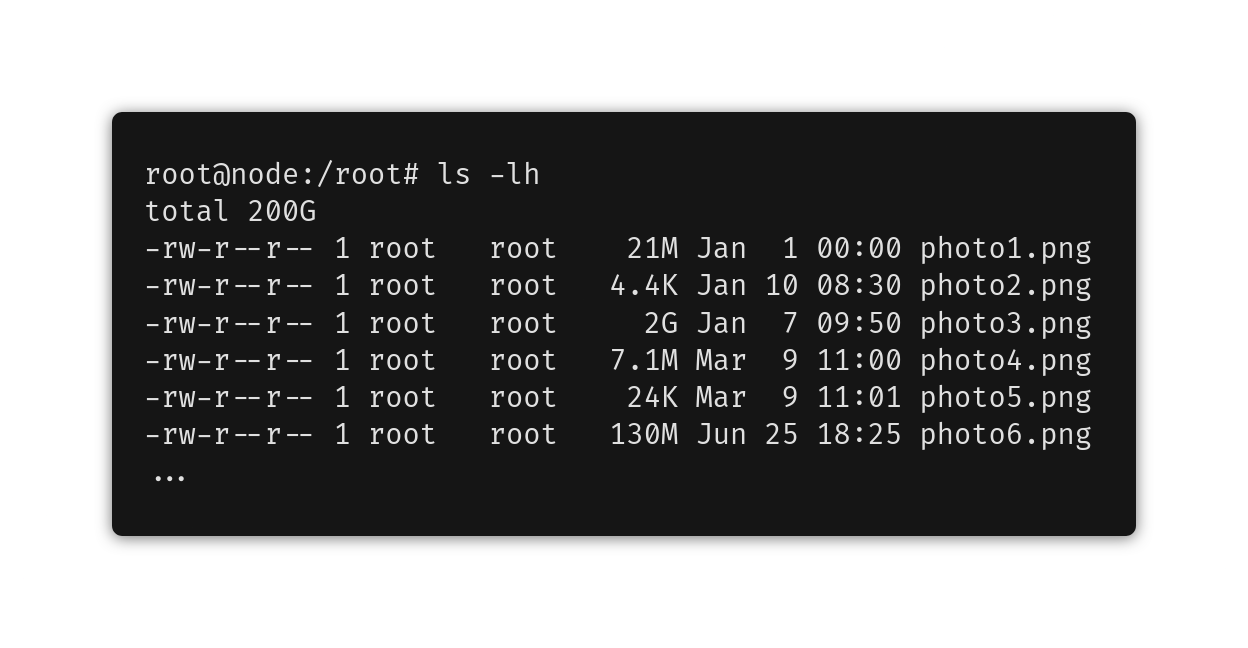
\includegraphics[width=0.8\linewidth]{static/shell-ls-problem.png}
        };

        % Calculate the width and height of the image node for later use
        \pgfgetlastxy{\imagewidth}{\imageheight}

        \coordinate (A) at ([xshift=.7cm, yshift=2.1cm]image.south west);
        \coordinate (B) at ([xshift=7.9cm, yshift=2.4cm]image.south west);

        \draw[red, very thick, line width=1pt]
            (A) rectangle (B);
    \end{tikzpicture}
\end{center}

We can use checksums.

\end{frame}

\begin{frame}{Problem}
    \begin{columns}[c]
        \begin{column}{0.4\textwidth}
            But, what if a file is split into pieces and distributed across different \textbf{regions}?
            \only{We would need to perform a checksum on each node.}
        \end{column}
        \begin{column}{0.6\textwidth}

            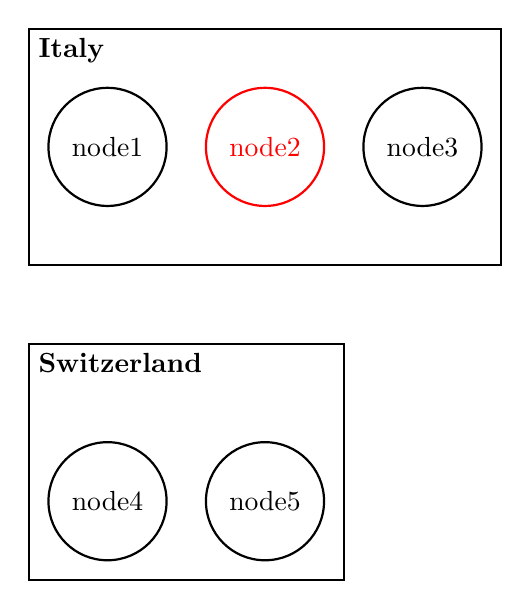
\begin{tikzpicture}
                \draw[thick] (0,0) rectangle (4,3);
                \node[anchor=north west] at (0,3) {\textbf{Switzerland}};
                \node[circle, draw, thick, minimum size=1.5cm] at (1,1) {node4};
                \node[circle, draw, thick, minimum size=1.5cm] at (3,1) {node5};

                \draw[thick] (0,4) rectangle (6,7);
                \node[anchor=north west] at (0,7) {\textbf{Italy}};
                \node[circle, draw, thick, minimum size=1.5cm] at (1,5.5) {node1};
                \node[circle, draw, red, thick, minimum size=1.5cm] at (3,5.5) {node2};
                \node[circle, draw, thick, minimum size=1.5cm] at (5,5.5) {node3};
            \end{tikzpicture}
        \end{column}
    \end{columns}
\end{frame}
